\begin{abstract}
 The abstract goes here...
\end{abstract}




%*****************************************
\chapter{Introduction}
%*****************************************
\hint{This chapter should motivate the thesis, provide a clear description of the problem to be solved, and describe the major contributions of this thesis. The chapter should have a length of about two pages!}

\section{Motivation}
What is the motivation for doing research in this area?

\section{Problem Statement and Contribution}
What is the problem that should be solved with this thesis?

\section{Outline}
How is the rest of this thesis structured?



%*****************************************
\chapter{Background}
\label{ch:background}
%*****************************************
\hint{This chapter should give a comprehensive overview on the background necessary to understand the thesis.
The chapter should have a length of about five pages!}


\section{Basics of Neural Networks\ \ \  \(WIP\)}
Neural networks are a part of most major AI-breakthrough in the last decade enabling computers to compete in fields formerly championed by humans.\footnote{
	\begin{itemize}
		\item 
			2011: "Watson" of IBM defeats two former grand champions in "Jeopardy!" \cite{lally2011natural}
		\item 
			2011: "Siri" enables users to use natural language to interact with their phones 
			\cite{ARON201124}
		\item 
			2015: A convolutional neural network classifies images from the ImageNet dataset more accurately than human experts 
			\cite{Russakovsky2015} \cite{He_2015_ICCV}
		\item 
			2016: "AlphaGo" beats Lee Sedol, one of the world's strongest Go players
			\cite{gibney2016google} \cite{silver2017mastering}
	\end{itemize}
}
They implement a statistical understanding of AI, which is to say that they try to find a specific model optimizing the likelihood of reproducing input-output pairs similar to some training data. The competing philosophy directly divines behaviour rules, frequently from expert knowledge, and as such is far less dependant from data.  
\textcolor{red}{[citation needed]}\\
For the former concept its model classes are the essential point of design. A multitude of properties maybe sought after in a model class of which a few important ones are:
\begin{itemize}
	\item \textbf{Richness:}\\
	The diversity of single models in the class and thus the ability to fit a wide field of different input-output landscapes.\footnote{
		More formally the richness of a model class can be described as the amount of different functions from the input-space to the output-space which can be expressed through a model of said class.}\\
	If a model class is inherently restricted the underlying relation between inputs and outputs might simply be beyond the expressive capabilities of all its models.\\
	In other words: If a model class is not rich enough all of its models will underfit the given training data.
	\item \textbf{Stability:}\\ 
	Tendency of similar models in the class to handle inputs in a similar way.\\
	If your model class shows unstable behavior defining a sensible way to search it for good models becomes difficult.
	\item \textbf{Interpretability of Models:}\\
	 Ease of formulating knowledge out of any given model in the class.\\
	 As fields exist in which statistical AI outperform experts the extraction of knowledge understandable and applicable by humans is of special interest.
	\item \textcolor{red}
	{[citation needed]}
\end{itemize}
If one knows an entity that already performs well on a given task it is a sensible approach to design ones model class to reproduce its decision process. Humans usually are such entities for many tasks of interest to AI research so they are a natural source of inspiration. Neural networks essentially are simplified models of a human central nervous system. \\
The most basic building block of the human central nervous system is a neuron which can receive multiple stimuli and is able to produce an output if the combined stimulation exceeds a threshold.\textcolor{red}{[citation needed]} One such neuron and its stimulus measure are depicted in \ref{fig:neuron1}. Another functionality observed in nature is the ability of a neuron to strengthen the connection to any source of stimulus thus giving said source more influence on whether the neuron produces an output. 
\textcolor{red}{[citation needed]}\\
\\
The canonical mathematical model of a neuron, as seen in \ref{fig:neuron2}, is defined as:
\begin{itemize}
	\item \textbf{Inputs} $x_i$ \textbf{:}\\
	All stimuli of a neuron are simply referred to as its inputs
	\item \textbf{Weights} $w_i$ \textbf{:}\\
	The ability to assign importances is modelled as weights which are coupled to specific stimuli
	\item \textbf{Combined Weighted Inputs} $\sum_{i=1}^{n}w_i x_i$ \textbf{:}\\
	After the inputs are scaled by their according weight they superpose to form the total excitation of the neuron
	\item \textbf{Activation Function} $\Phi(\sum_{i=1}^{n}w_i x_i)$ \textbf{:}\\
	...
	\item \textbf{Bias} $b$ \textbf{:}\\  
	...
\end{itemize}


\begin{figure}
	\centering
	\begin{minipage}{0.45\textwidth}
		\centering
		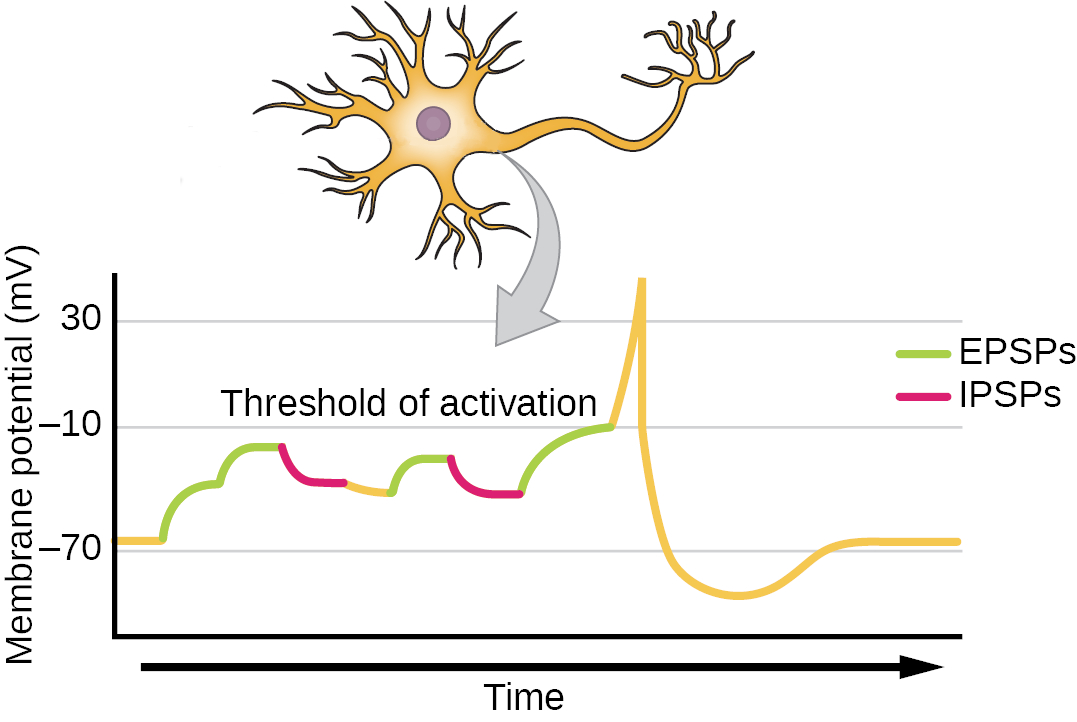
\includegraphics[height=150px]{gfx/Biological_Neuron_edited.jpg}
		\caption{Representation of a biological Neuron\\
			\cite{biology} edited}
		\label{fig:neuron1}
	\end{minipage}\hfill
	\begin{minipage}{0.45\textwidth}
		\centering
		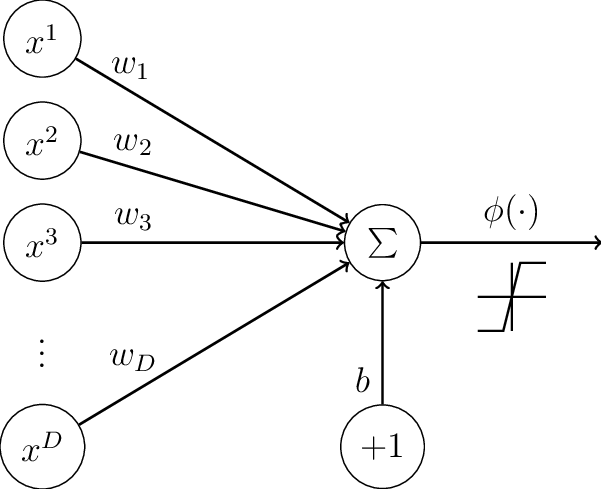
\includegraphics[height=150px]{gfx/Abstract_Neuron.png}
		\caption{Abstraction of a Neuron\\
			\cite{abstract_neuron}}
		\label{fig:neuron2}
	\end{minipage}
\end{figure}

As an individual neurons is too simple to model any complex relations between inputs
and outputs the next step is to aggregate multiple neurons. Figure \ref{fig:FFNetwork} displays a few neurons coming together to form a simple fully-connected feed-forward network.
\footnote{
	Inputs of neural networks are often called "features" and fully-connected networks are frequently referred to as "dense"	}
\begin{figure}
	\centering
		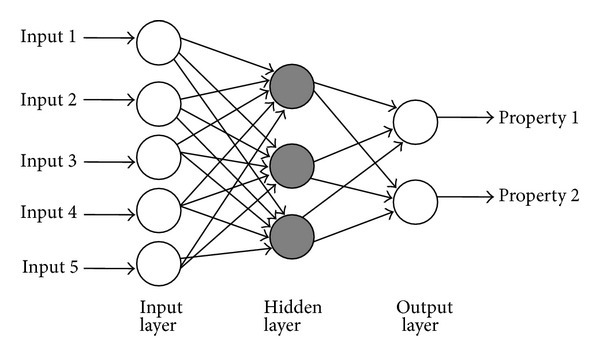
\includegraphics[height=150px]{gfx/Dense_FFNetwork.jpg}
		\caption{A small fully-connected network\\
			\cite{dense_network}}
		\label{fig:FFNetwork}
\end{figure}

\begin{itemize}
	\item \textcolor{red}{TODO:}
	\item Issue of computational expense
	\item CNNs (and other forms of NN?)
\end{itemize}
	
\section{The Lottery Ticket Hypothesis}
\begin{itemize}
	\item \textcolor{red}{TODO:}
	\item Issue of overloading on parameters
	\item Clarifying the task (image classification)
	\item Idea of trainable subnets
\end{itemize}

\section{Basics of Natural Language Processing}
\begin{itemize}
	\item \textcolor{red}{TODO:}
	\item (?) Corpora
	\item Tokenizing
	\item Language Models
	\item (?) Handeling missing words in the Language model
\end{itemize}

\section{Combining LMs \& CNNs}
\begin{itemize}
	\item \textcolor{red}{TODO:}
	\item Interpreting the tensor representation of a sentence/document as an image to be classified
	\item (?) Validation through results
	\item (?) Handeling different sizes of inputs
\end{itemize}


%*****************************************
\chapter{Related Work}
\label{ch:relatedwork}
%*****************************************
To quantify the goals previously defined the context of current research is needed. The importance of any work assuming an underlying architecture can not be correctly evaluated without knowledge about the quality of said architecture. As such this section shortly presents state-of-the-art approaches to the tasks relevant to this thesis. Additionally an overview over previous compression methods and their achievements is given. Furthermore the difference between image classification on the MNIST-dataset and topic classification on the Reuters-21578-dataset, as staple tasks of their respective fields, is specified. At the end of this section reasons are given why the collected related work does not yet satisfy the discussed goals.


\section{Image Classification: MNIST}
The MNIST-dataset contains 70.000 datapoints encoding 28x28-gray-scale-images of which 60.000 are designated for training and 10.000 for validation. The task is classification of a datapoint into one of ten digit-classes \cite{MNIST}.\\
Currently the best performing system combines fully connected, convolutional  and long-short-term-memory networks achieving a 0.18\% error-rate \cite{RMDL}. Multiple approaches share second place with an error-rate of 0.20\% correctly classifying 2 fewer examples \cite{Multi-Column} \cite{APAC} \cite{Batch-Normalized} \cite{ReNet} \cite{Keep-It-Simple}. Restricted to simple models the lowest error-rate is achieved by a pruned fully-connected architecture with 2 hidden layers (300-100-Lenet) at 1.26\% \cite{Sparse-From-Sratch}.
\footnote
	{State-of-the-Art architectures are presented as described on \href{https://paperswithcode.com/sota}{https://paperswithcode.com/sota}}\\
While J. Frankle \& M. Carbin do not provide exact values their figures indicate that the fully-connected Lenet-Architecture they study achieves roughly 98\% accuracy on the test-data which translates to an error-rate of 2\% and about 200 wrongly classified datapoints out of 10000 \cite{Frankle2018}. This result is reproducible with the source code provided alongside this thesis.

\section{Pruning}
Beginning around 1990 with M.C. Mozer \& P. Smolensky \cite{Skeletonization} as well as LeCun et al. \cite{Optimal-Brain-Damage} weights were being removed from neural networks after training them for a task. Shortly thereafter the idea of further training a pruned network was proposed \cite{Optimal-Brain-Surgeon} which became common practice over the next decade. While LeCun et al. describe a network compression factor of $\times4$, more recent works achieve a factor of $\times9$ to $\times16.6$ while loosing no or close to no accuracy \cite{Learning_Weights_And_Connections} \cite{ThiNet}.\\
In their paper on the Lottery-Ticket-Hypothesis (now LTH) J. Frankle \& M. Carbin report pruning over 98,5\% of weights in one of their networks while maintaining network capabilities which amounts to a compression rate of over $\times50$


\section{Topic Classification: Reuters-21578}
The Reuters-21578-dataset contains 21578 articles published by the Reuters News Agency in 1987 \cite{Reuters-21578}. Reuters-21578 differs from MNIST in the sense that it lacks a few fundamental properties. In particular Reuters-21578 is not only multi-class but rather multi-label meaning that any one data point can satisfy multiple categories. Additionally there are categories in Reuters-21578 that have no associated positive example and even for all remaining ones the amount of samples is heavily skewed. In order to restore parts of the missing properties with minimal change to the dataset different subsets of Reuters-21578 have been chosen by different researchers.\\
F. Debole \& F. Sebastiani \cite{Reuters-Subsets} describe those subsets, starting out with the fact that close to half of the data points are unusable leaving 12,902 documents. 9,603 are marked for training and 3,299 for validation.\footnote{While different training-splits were proposed for Reuters-21578 "ModApt\'e" has become the canonical choice} They also point out the different groups of categories used for classification:
\begin{itemize}
	\item \textbf{R$\left(115\right)$}\\
	The group with the 115 categories with at least one positive training example.\\ 
	\item \textbf{R$\left(90\right)$}\\
	The group with the 90 categories with at least one positive training and test example.\\ 
	\item \textbf{R$\left(10\right)$}\\
	The group with the 10 categories with the most examples. \\
\end{itemize} 
State of the art approaches to Reuters-21578 topic classification consist of Long-Short-Term-Memory \cite{Rethinking-LSTM} or mixed architectures \cite{RMDL} achieving an F1-score of 0.87 and 90.69\% accuracy respectively.

\section{Topic Classification: Convolutional Neural Networks For NLP}
While the LTH is not yet extended to Long-Short-Term-Memory architectures there are approaches to NLP-tasks  which are more closely aligned with computer vision. In a paper from 2014 \cite{CNN-For-NLP} Y. Kim describes how a simple convolutional neural network architecture, utilizing word embedding through language model, demonstrates capabilities similar to state-of-the-art approaches for various NLP-tasks.

\section{Early Pruning}
In a recent paper \cite{Rethinking-Network-Pruning} Z.Liu et al. observe that if pruned networks are trained with randomly reinitialized weights instead of fine-tuning their previous ones they retain from the original network, the pruned networks keep their capabilities. They conclude that said weights can not be essential to a pruned networks quality, contrary to prior common belief. Thus Z.Liu et al. claim that the architecture of pruned networks is responsible for its capabilities and furthermore that pruning can be interpreted as a kind of network architecture search .\\
After the effectiveness of pruning is established and its interpretation as network architecture search becomes available there is a legitimate question whether all the weights in a network are really necessary for all of the training. In a paper of Y. Li \& W. Zhao \& L. Schang from early 2019 \cite{Pruning-With-Little-Training} they describe a method named IPLT to prune common convolutional network architectures at the filter level and especially before convergence. Thus they do not only compress the networks by a factor of $\times10$ but also speed up training by a similar magnitude. 

\section{Additions to the Lottery Ticket Hypothesis}
Even though the Lottery-Ticket-Hypothesis was only proposed earlier this year additional papers on the topic exist.
In a paper from June 2019 J. Frankle \& M. Carbin et al. \cite{LTH-At-Scale} expand their method to find winning tickets on deep convolutional network architectures that proved difficult before. They attribute this achievement to the decision of not returning to the very first state of the network but to one a few iterations into training.\\
Additionally H. Zhou et al. \cite{Deconstructing_LTH} document an ablation study on the phenomenon of lottery tickets. They reaffirm the initially naive magnitude-based pruning and describe "supermasks" that improve accuracy when applied to the initial network even without additional training. Finally they find that a replacement of all weights in the pruned network by a constant with same sign as said weights does not significantly influence the networks capabilities. As such H. Zhou et al. conclude that the sign of weights are the essential property for such neural networks. 


\section{Task in context of Related Work}
To conclude this chapter the given information about related work is interpreted in regards to the three defined subtasks: 
\begin{itemize}
	\item \textbf{1. Reproduction}\\
	Reproduction of the LTH is highly independent of the related work mentioned so far.\footnote{Side note: While tensorflow 1.x source code exists at \href{https://paperswithcode.com}{https://paperswithcode.com}, for the first LTH-paper, tensorflow 2.0 is much easier to operate and code for so rebuilding the framework is still valuable.}\\ 
	\item \textbf{2. Extending to NLP}\\
	Even though the LTH has not yet been applied to Long-Short-Term-Memory architectures and doing so is beyond the scope of this thesis the question whether it can hold for a more disorderly dataset at all is still open and of interest. The approach described in 3.4 is generally applicable to the Reuters-21578 dataset as well as already performing well on other NLP-tasks while also being compatible with the current Application of the LTH.\\ 
	\item \textbf{3. Early pruning}\\
	While IPLT \cite{Pruning-With-Little-Training} already provides an early pruning approach the LTH has shown capabilities of much stronger compression. While this compression does not yield any speed-up yet because unstructured sparse layers need a special infrastructure to accelerate, verification of so significant compressions rates found by the LTH early in training might motivate such infrastructures.\\
\end{itemize} 

%*****************************************
\chapter{Design}
\label{ch:design}
%*****************************************
\hint{This chapter should describe the design of the own approach on a conceptional level without mentioning the implementation details. The section should have a length of about five pages.}

\section{Requirements and Assumptions}

\section{System Overview}

\subsection{Component 1}

\subsection{Component 2}

\section{Summary}

%*****************************************
\chapter{Implementation}
\label{ch:implementation}
%*****************************************

\hint{This chapter should describe the details of the implementation addressing the following questions: \\ \\
1. What are the design decisions made? \\
2. What is the environment the approach is developed in? \\
3. How are components mapped to classes of the source code? \\
4. How do the components interact with each other?  \\
5. What are limitations of the implementation? \\ \\
The section should have a length of about five pages.}
\section{Design Decisions}

\section{Architecture}

\section{Interaction of Components}

\section{Summary}

%*****************************************
\chapter{Evaluation}
\label{ch:evaluation}
%*****************************************
\hint{This chapter should describe how the evaluation of the implemented mechanism was done. \\ \\
1. Which evaluation method is used and why? Simulations, prototype? \\
2. What is the goal of the evaluation? Comparison? Proof of concept? \\
3. Wich metrics are used for characterizing the performance, costs, fairness, and efficiency of the system?\\
4. What are the parameter settings used in the evaluation and why? If possible always justify why a certain threshold has been chose for a particular parameter.  \\
5. What is the outcome of the evaluation? \\ \\
The section should have a length of about five to ten pages.}
\section{Goal and Methodology}

\section{Evaluation Setup}

\section{Evaluation Results}

\section{Analysis of Results}


%*****************************************
\chapter{Conclusions}
\label{ch:closure}
%*****************************************

\hint{This chapter should summarize the thesis and describe the main contributions of the thesis. Subsequently, it should describe possible future work in the context of the thesis. What are limitations of the developed solutions? Which things can be improved?
The section should have a length of about three pages.}

\section{Summary}

\section{Contributions}

\section{Future Work}

\section{Final Remarks}
